\newpage
\phantomsection
\chapter{Análisis de Producto de Mercado}
\section{Estudio de mercado}

    \phantomsection
    \subsection{Descripción del área geográfica que abarca el mercado del proyecto}
    
        El mercado objetivo se localiza en la Provincia de Misiones, Argentina. Se enfoca principalmente en los centros urbanos con mayor infraestructura oftalmológica (como Posadas, Oberá y Eldorado), donde se concentran las clínicas privadas y hospitales públicos que cuentan con equipos de diagnóstico de alta complejidad (Pentacam, Sirius, etc.). Al ser los lugares de mayor densidad poblacional de la provincia, en ellos se concentra la mayor parte del diagnostico oftalmológico, en donde se pretende implementar un soporte para la diferenciar entre la enfermedades oculares comunes y el queratocono. 

    \phantomsection
    \subsection{Descripción de los bienes y/o servicios que provea el proyecto}
    
        El proyecto proveerá un \textit{software} como producto médico que ofrece un servicio de soporte a la decisión clínica, el cual busca disminuir subjetividades por parte del especialista sirviendo como una ``segunda opinión experta''. Donde las funciones principales incluirían:
        
        \begin{itemize}[leftmargin=*]
            \item \textbf{Análisis automatizado:} Procesamiento de imágenes de mapas topográficos y datos clínicos.
            
            \item \textbf{Estratificación de riesgo:} Clasificación basada en el sistema ABCD de Belin.
            
            \item \textbf{Explicabilidad (XAI):} Generación de mapas de calor que justifiquen la predicción del algoritmo.
            
            \item \textbf{Reportes:} Generación de un informe detallado con el resultado de la inferencia y niveles de fiabilidad.
        \end{itemize}

        \begin{figure}[H]
            \centering
            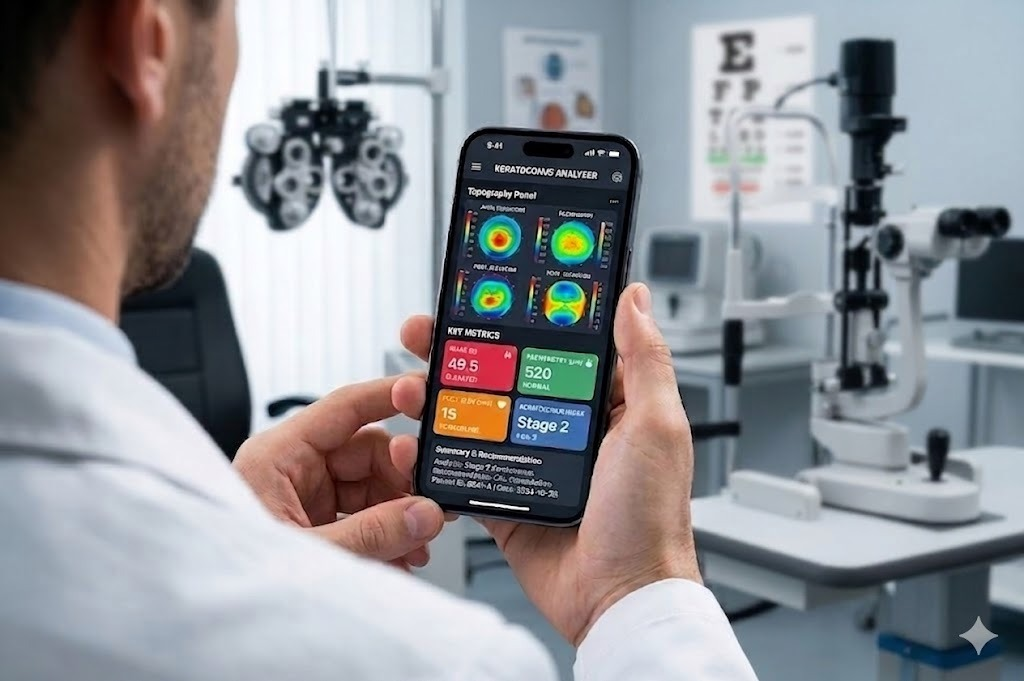
\includegraphics[width=0.5\linewidth]{img/humo.jpeg}
            \caption{Representación visual de la aplicación.}
        \end{figure}

    \phantomsection
    \subsection{Descripción de los usuarios y usos posibles}
    
        \subsubsection*{Usuarios}
    
            Los usuarios destinatarios corresponderían a los médicos oftalmólogos generales, especialistas en córnea y técnicos en centros de optometría de alta complejidad, los cuales dispongan del equipo necesario para la realización de los estudios.
    
        \subsubsection*{Usos Posibles}
    
            \begin{itemize}
                \item Detección temprana de queratocono subclínico en pacientes jóvenes.
                
                \item Estandarización de criterios diagnósticos en la interpretación de mapas corneales.
            \end{itemize}

        \subsection{Análisis de demanda}
        
            Aunque no se manifieste una demanda excesiva de una herramienta de soporte a la decisión por parte de los profesionales, existe una necesidad creciente por la misma, resultante de la naturaliza subjetiva de los análisis  de los estudios. Estos son dependientes de la experiencia de los oftalmólogos, lo cual aumenta la probabilidad de cometer errores en la detección, sobre todo en etapas subclínicas, es decir, etapas iniciales donde la manifestación suele confundirse con enfermedades mas comunes y menos nocivas~\citeB{deteccion_temprana}. 
            
            En este apartado el producto ofrece la capacidad de mitigar dicha subjetividad al actuar como una ``segunda opinión experta'', reduciendo la dependencia de la experiencia del médico de turno, garantizando un diagnóstico preciso y estandarizado independientemente de quién evalúe el estudio.
            
            Esto descentralizaría, en cierta medida, la atención médica de alta complejidad, un factor especialmente crítico en provincias o zonas alejadas de las grandes capitales generando interés enorme para centros médicos regionales derivando a los centros de alta complejidad únicamente los casos que realmente lo requieren. 
            
            La demanda se sustenta en:
            
            \begin{itemize}
                \item La necesidad de reducir el margen de error diagnóstico~\citeB{deteccion_temprana}.
                
                \item El alto volumen en Misiones de afectados que requieren el diagnóstico preciso de la patología~\citeB{misiones}.  
                
                \item El respaldo de normativas para la modernización tecnológica en salud pública y privada~\citeB{dispo_2318,dispo_9688}.
            \end{itemize}

        \phantomsection
        \subsection{Análisis de la oferta}

            El mercado global está dominado por un grupo reducido de empresas que comercializan sistemas cerrados, los cuales analizan y reestructuran los datos provenientes de los mismos equipos sin realizar predicciones ni diagnósticos sobre los mismos, donde el software de análisis depende obligatoriamente de tener sus dispositivos propietarios. A nivel nacional, no existen competidores directos con un software como producto médico específico para queratocono. La Tabla~\ref{tabla:oferta_cualitativa} resume las características cualitativas de los competidores identificados.

            \begin{longtblr}[
                caption = Características cualitativas de la oferta competitiva,
                label = tabla:oferta_cualitativa
                ]{
                    cells={ valign = m, halign = l }, 
                    colspec = {Q[l, 3 cm] Q[l, 6 cm] Q[l, 6 cm]}, 
                    rowsep = 4 pt,        
                    colsep = 5 pt,           
                    hlines,              
                    vlines,                             
                    row{1}={bg=gray!15, font=\bfseries, halign = c}
                }
                
                Competidor & Descripción & Limitación \\
                
                Oculus (Familia Pentacam) 
                & Referente del sector. Oferta desde modelos básicos hasta el Pentacam AXL Wave con biometría y wavefront~\citeB{oculus}. 
                & Sistema cerrado. Software dependiente de hardware propietario. \\

                Topcon Healthcare 
                & Conectividad mediante Harmony e IDHea. Integra datos de topógrafos de Placido (CA-800) para análisis longitudinal asistido por IA~\citeB{topcon}. 
                & Sistema cerrado. Sin módulo específico para queratocono. \\

                KERAFound (Dr. Shafi Balal / Moorfields) 
                & Plugin de código abierto en desarrollo para predecir riesgo de progresión del queratocono~\citeB{shafi_balal}. 
                & En fase de investigación. Sin integración a sistemas médicos. \\

                KeratoDetect 
                & Algoritmo CNN para detección binaria subclínica~\citeB{kerato_detect}. 
                & Código cerrado. Solo detección, sin estratificación ni integración. \\

                AEYE 
                & Sistema multi-agente de IA para detección de queratocono y evaluación de elegibilidad refractiva~\citeB{aeye}. 
                & Diseñado para sistemas internacionales de alta gama. \\

                Entelai 
                & Startup Argentina para análisis de imágenes médicas con IA~\citeB{entelai}. 
                & Solución general. Sin módulo específico para queratocono. \\

                \textbf{Nuestro proyecto} 
                & Software independiente (SaMD) multimodal. Detección temprana + estratificación de riesgo en sistema abierto y accesible. 
                & Desarrollo acotado a normativas ANMAT. Necesidad de validación local. \\
                
            \end{longtblr}

        \phantomsection
        \subsection{Análisis de precios}

            La Tabla~\ref{tabla:precios_cuantitativa} presenta la comparativa de precios y costos de los competidores identificados, diferenciando entre inversión inicial, modelo de facturación y costo por uso.

            \begin{longtblr}[
                caption = Comparativa de precios y costos de la oferta competitiva,
                label = tabla:precios_cuantitativa
                ]{
                    cells={ valign = m, halign = l }, 
                    colspec = {Q[l, 3.5 cm] Q[l, 4 cm] Q[l, 4.5 cm]}, 
                    rowsep = 4 pt,        
                    colsep = 5 pt,           
                    hlines,              
                    vlines,                             
                    row{1}={bg=gray!15, font=\bfseries, halign = c}
                }
                
                Competidor & Inversión inicial & Modelo de facturación \\
                
                Sistemas Tradicionales (Oculus/Ziemer) 
                & USD $ \$\,20.000$ a USD $ \$\,40.000$ por equipo + software 
                & Licencia cerrada e inflexible \\

                Referente IA Local (Entelai) 
                & No requiere hardware propio 
                & SaaS / Pay-per-scan: $\approx \$\,3.790 + IVA$ por informe~\citeB{entelai} \\

                \textbf{Nuestra Propuesta} 
                & No requiere hardware nuevo. Procesa imágenes de cualquier equipo estándar 
                & Suscripción mensual SaaS \\
                
            \end{longtblr}

            \subsubsection*{Estructura de costos del proyecto}
            
            \begin{itemize}[leftmargin=*]
                \item \textbf{Infraestructura Mensual:} Aproximadamente $ \$\,41.600\:ARS$. Esto incluye el servidor VPS (KVM 4 de Hostinger a $\approx \$\, 23.300$) y la plataforma de entrenamiento (Google Colab Pro a $\approx \$\,18.300$ con impuestos incluidos).  
    
                \item \textbf{Validación Médica:} El costo operativo por hora de un especialista para auditoría de datos es de $\approx\$\,30.000 \: ARS$.  
    
                \item \textbf{Barrera Regulatoria (ANMAT):} El registro del producto Clase II cuesta $\$\,52.000 \:ARS$, pero la habilitación inicial de la empresa como fabricante/importador requiere un pago único de $ \$\,1.523.100 \:ARS$.
            \end{itemize}

        \phantomsection
        \subsection{Análisis de la comercialización}
        
            \subsubsection{Definición del producto requerido por los consumidores potenciales}
        
            Los oftalmólogos ``demandan'' una herramienta que sea:
        
            \begin{itemize}
                \item \textbf{Interoperable:} Capaz de recibir imágenes de distintos dispositivos diagnósticos.  
        
                \item \textbf{Intuitiva:} Con una interfaz amigable (React) que no requiera conocimientos técnicos en IA.  
        
                \item \textbf{Fiable:} Que proporcione evidencia visual (XAI) para sustentar la decisión clínica ante el paciente.
            \end{itemize}
        
            \subsubsection{Estrategia de comunicación de los consumidores potenciales}
        
            La estrategia de comunicación para incentivar la adopción por parte de los consumidores potenciales (clínicas, centros de salud y oftalmólogos) se estructurará en los siguientes focos:
        
            \begin{itemize}
                 \item \textbf{Mensaje central y propuesta de valor:} Difusión de los beneficios clave del sistema (estandarización clínica y optimización de recursos), posicionándolo como una ``segunda opinión'' que reduce la subjetividad en análisis topográficos y tomográficos, previniendo errores en etapas subclínicas.  
            
                \item \textbf{Difusión científica:} Publicación de resultados de la validación con datos locales en congresos regionales o internacionales de oftalmología o informática.  
        
                \item \textbf{Marketing directo:} Presentaciones institucionales en clínicas privadas de Misiones, el Ministerio de Salud Pública o interesados.  
        
                \item \textbf{Presencia digital y educativa:} Difusión en redes profesionales (LinkedIn), envío de newsletters especializados del sector salud y organización de webinars técnicos para la adopción y actualización continua de los profesionales.
            \end{itemize}
        
            \subsubsection{Estrategia de venta y distribución del producto}
        
                La estrategia de venta y distribución para el software se centra en un modelo de servicio digital escalable, diseñado para integrarse de manera directa en el flujo de trabajo del oftalmológico actual. El objetivo es facilitar el acceso al soporte diagnóstico mediante una infraestructura en la nube práctica, rápida y eficaz, planteando a la herramienta como un complemento para el equipamiento diagnóstico tradicional.

            \vspace{-0.5 cm}
            \paragraph{Distribución y acceso:}
            
            \begin{itemize}
                \item El software se desplegará en un servidor VPS.
                
                \item El acceso al usuario final mediante una plataforma web o una aplicación móvil desarrollada en React Native, permitiendo al oftalmólogo consultar los resultados desde cualquier dispositivo.
            \end{itemize}

            \vspace{-0.5 cm}
            \paragraph{Canales de venta:}
            
            \begin{itemize}
                \item Venta directa a instituciones de salud.  
                
                \item Colaboración con distribuidores de equipamiento oftalmológico para ofrecer el software como un valor agregado (plugin) a sus equipos.  
                
                \item Asistencia técnica remota para garantizar el mantenimiento y actualización del sistema.
            \end{itemize}

        \phantomsection
        \subsection{Estudio de factibilidad y viabilidad del proyecto}
        
            \subsubsection*{Criterios de ponderación}
        
            \paragraph{Viabilidad técnica} (40\% de influencia) Determina si el equipo de desarrollo cuenta con los recursos y experiencia para cumplir los requisitos.
        
            \begin{itemize}
                \item \textbf{Accesibilidad de tecnologías y datos:} Evaluar la facilidad para obtener \textit{hardware} de entrenamiento, herramientas de \textit{software} y el acceso a los datasets multimodales.
        
                \item \textbf{Capacidad técnica del equipo:} Medir si los integrantes poseen las habilidades necesarias en \textit{Deep Learning}, desarrollo \textit{backend/frontend} y manejo de normativas médicas.
        
                \item \textbf{Interoperabilidad:} Capacidad del sistema para integrarse con diferentes equipos de diagnóstico (Pentacam, Sirius).
        
                \item \textbf{Mantenibilidad del sistema:} La facilidad con la que el software puede ser actualizado, corregido o adaptado a nuevas versiones o cambios en los formatos de salida de los equipos de diagnóstico.
            \end{itemize}
        
            \paragraph{Viabilidad jurídica} (25\% de influencia) Para asegurar el cumplimiento normativo respecto a la salud.
        
            \begin{itemize}
                \item \textbf{Cumplimiento de normativas ANMAT:} Factibilidad de registrar el software como producto médico (SaMD) bajo las disposiciones 2318/02 \citeB{dispo_2318} y 9688/19 \citeB{dispo_9688}, clasificándolo como clase II.  
                
                \item \textbf{Protección de datos personales:} Garantizar que los procesos de anonimización de datos locales cumplan con la Ley 25.326 \citeB{ley_25326} de Protección de Datos Personales.  
                
                \item \textbf{Consentimiento informado:} Viabilidad de gestionar los permisos legales necesarios con los pacientes de Misiones para el uso de sus muestras en la validación.
            \end{itemize}

            \vspace{-0.5 cm}
            \paragraph{Viabilidad operativa} (20\% de influencia) Analizar si el sistema se utilizará y funcionará al instalarse.
        
            \begin{itemize}
                \item \textbf{Predisposición y aceptación del usuario:} Nivel de apertura de los oftalmólogos para adoptar herramientas de IA como apoyo diagnóstico.  
                
                \item \textbf{Facilidad de uso e interfaz:} Evaluación de si la curva de aprendizaje de la aplicación es lo suficientemente baja para el personal médico con poca experiencia en el uso de herramientas digitales.  
                
                \item \textbf{Integración al flujo de trabajo:} Determinar si el sistema agiliza o entorpece la consulta diaria del especialista. 
            \end{itemize}

            \vspace{-0.5 cm}
            \paragraph{Viabilidad económica} (15\% de influencia) Evalúa la rentabilidad y la capacidad de solventar los gastos.
        
            \begin{itemize}
                \item \textbf{Costos directos de desarrollo e implementación:} Incluye licencias de plataformas de desarrollo (Colab Pro por ejemplo), \textit{hosting} VPS y los aranceles de ANMAT.  
                
                \item \textbf{Costos de validación clínica:} Honorarios de los especialistas médicos por las horas dedicadas a auditar el sistema o consultas pertinentes.  
                
                \item \textbf{Relación costo beneficio:} Compara el esfuerzo económico invertido frente al valor o ahorro que el proyecto generará a largo plazo a los especialistas.
            \end{itemize}
        
            \subsubsection*{Análisis por criterio}
        
            \paragraph{Viabilidad técnica}
        
            \begin{itemize}
                \item \textbf{Accesibilidad de tecnologías y datos:} El queratocono dispone de \textit{datasets} públicos y privados de mayor accesibilidad, junto a una disponibilidad de datos locales alta.
        
                \item \textbf{Capacidad técnica del equipo:} El desarrollo posee implementaciones previas similares en un ambito académico en herramientas e implementación por parte del equipo.
        
                \item \textbf{Interoperabilidad:} El queratocono utiliza mapas y datos topográficos mas estandarizados.
        
                \item \textbf{Mantenibilidad del sistema:} Se presenta mayor en el queratocono dada la menor demanda de almacenamiento y procesamiento.
            \end{itemize}
        
            \paragraph{Viabilidad jurídica} 
        
            \begin{itemize}
                \item \textbf{Cumplimiento de normativas ANMAT:} El desarrollo se categoriza como producto médico clase II. Debido al riesgo asociado al diagnóstico, la ANMAT exigirá demostrar que el modelo es robusto.
                
                \item \textbf{Protección de datos personales:} Los datos oftalmológicos presentan un menor riesgo de sensibilidad bajo la Ley 25.326 \citeB{ley_25326}.
                
                \item \textbf{Consentimiento informado:} Es más factible de gestionar logísticamente en clínicas de oftalmología.
            \end{itemize}
        
            \paragraph{Viabilidad operativa} 
        
            \begin{itemize}
                \item \textbf{Predisposición y aceptación del usuario:} Alta en el proyecto, ya que los oftalmólogos muestran una necesidad de asistencia debido al valor que existiría ante una herramienta capaz de agilizar tiempos de espera en diagnósticos de pacientes con esta patología.
                
                \item \textbf{Facilidad de uso e interfaz:} La interfaz busca ser intuitiva para personal no técnico.
                
                \item \textbf{Integración al flujo de trabajo:} El sistema de queratocono se podría insertar mas fluidamente en la consulta dado el carácter mas digital de los equipos.
            \end{itemize}
        
            \paragraph{Viabilidad económica}
        
            \begin{itemize}
                \item \textbf{Costos directos de desarrollo e implementación:} El queratocono requiere infraestructura estándar.
                
                \item \textbf{Costos de validación clínica:} Menor en costo y tiempo para el queratocono.
                
                \item \textbf{Relación costo beneficio:} El queratocono evitaría trasplantes y proporcionaría una identificación temprana con un software de menor mantenimiento.
            \end{itemize}

    \vspace{-0.5 cm}
    \phantomsection
    \section{Presupuesto}

        \phantomsection
        \subsection{Recursos materiales}

            Al tratarse de un software como producto médico, los insumos requeridos son exclusivamente digitales. Afortunadamente, se obtendrán a través de vías institucionales o de código abierto, por lo que no representan un costo económico:

            \begin{itemize}
                \item \textbf{Muestras locales:} Lote de $150$ imágenes de topografías corneales anonimizadas, provistas por el consultorio médico asociado para realizar la validación clínica local de los algoritmos.
    
                \item \textbf{Datasets de información:} Bases de datos públicas e internacionales con casos de queratocono, las cuales se utilizarán en la etapa de entrenamiento inicial de la Inteligencia Artificial.
            \end{itemize}

            \begin{itemize}
                \item \textbf{Computadoras portátiles (\textit{Notebooks}):} Se requiere \textit{hardware} estándar para las tareas de programación y desarrollo local durante la ejecución del proyecto, así como para eventuales ajustes o mantenimientos futuros. Tomando como referencia equipos con procesador Intel Core i7 y 16 GB de RAM, el valor de mercado actual ronda entre los $\$\,1.800.000$ y $\$\,2.100.000$ ARS por unidad. Teniendo en cuenta que se planea adquirir estos equipo para el desarrollo exclusivo de este proyecto, uno por cada integrante, el costo total estimado es de $\$\,4.200.000$.
            \end{itemize}

        \phantomsection
        \subsection{Recursos humanos}

            El desarrollo del proyecto sera llevado a cabo tanto por mano de recursos humanos propios, como también por parte de personal adicional o externo para las áreas de marketing y diseño. La estructura de los recursos humanos es la siguiente:
    
            \subsubsection*{Recursos humanos propios}
    
                Los valores calculados a continuación se basan en los honorarios recomendados por el Consejo Profesional de Ciencias Informáticas de Córdoba \citeB{honorarios_profesionales_cordoba}. Sin embargo, para garantizar la viabilidad del proyecto, se asignaron retribuciones simbólicas basadas en el valor de un salario Mínimo Vital y Móvil (SMVM) \citeB{cita:SMVM} en proporción a una jornada laboral de cuatro horas diarias.
                
                \begin{itemize}
                    \item \textbf{Programador Inteligencia Artificial:} Este rol es el principal encargado del desarrollo y entrenamiento del modelo en la primer fase del proyecto. Con una participación de 9 meses y dedicación del 50\%, el costo total, basado en su retribución simbólica, estimado es de $\$\,3.171.600$.
        
                    \item \textbf{Desarrollador Web Full Stack:} Este rol comienza a desarrollarse en la segunda fase del proyecto, correspondiente a la implementación e integración. Se encargará del desarrollo del \textit{backend} y \textit{frontend} de la aplicación. Con una participación de 2 meses y dedicación del 50\% el costo total, basado en su retribución simbólica, estimado es de $\$\,704.800$.
                \end{itemize}
    
            \subsubsection*{Recursos humanos adicionales}
                
                Los valores calculados a continuación se basan en el salario mediano de dichos roles (\citeB{cita:salario_marketing} y  \citeB{cita:salario_UX_UI}).
                
                \begin{itemize}
                    \item \textbf{Diseñador UX y UI:} Su actividad se centrará en la segunda fase, de implementación e integración junto a los desarrolladores web, diseñando interfaces intuitivas y amigables para que sea simple de usar para usuarios no técnicos. Con una participación de 1 meses y dedicación del 30\% el costo total estimado es de $\$\,480.800$.
        
                    \item \textbf{Especialista en marketing digital:} Este perfil se enfocará en la creación de compañas de marketing digital y en realizar sugerencias  en cuanto a la información presentada en \textit{newsletters}, \textit{webinars} y congresos científicos. Con una participación de 1 meses de dedicación del 20\% el costo total estimado es de $\$\,162.000$.
                \end{itemize}

            \vspace{-0.25 cm}
            \begin{longtblr}[
                caption = Recursos humanos propios que intervendrán en el proyecto,
                label = tabla:rrhh_propios
                ]{
                    cells={ valign = m, font = \footnotesize },
                    colspec = {
                    Q[l, 3.9 cm] Q[c, 1.2 cm] Q[r, 2.25 cm] Q[r, 2.25 cm] Q[c, 1.5 cm] Q[c, 1.3 cm] Q[r, 2.2 cm] 
                    },
                    rowsep = 4 pt,
                    colsep = 3 pt,
                    hlines,
                    vlines,
                    row{1}={bg=gray!15, font=\bfseries\footnotesize, halign = c},
                    row{4}={bg=gray!15, font=\bfseries\footnotesize}
                }
            
                Profesión / función en el proyecto & Cant. & Costo mensual real c/u & Retribución simbólica & Meses de partic. & \% de dedic. & Costo total \\
            
                Programador IA & 2 & $\$\,3.783.577,52$ & $\$\,352.400,00$ & 9 & 50 & $\$\,3.171.600,00$ \\
            
                Desarrollador Web Full Stack & 2 & $\$\,3.453.169,23$ & $\$\,352.400,00$ & 2 & 50 & $\$\,704.800,00$ \\
            
                \SetCell[c=6]{r} TOTAL & & & & & & $\$\,3.876.400,00$ \\
            
            \end{longtblr}

            \vspace{-0.75 cm}
            \begin{longtblr}[
                caption = Recursos humanos adicionales requeridos en el proyecto,
                label = tabla:rrhh_adicionales
                ]{
                    cells={ valign = m, font = \small },
                    colspec = {Q[l, 2.4 cm] Q[l, 4.6 cm] Q[r, 2.5 cm] Q[c, 1.5 cm] Q[c, 1.4 cm] Q[r, 2.3 cm]},
                    rowsep = 4 pt,
                    colsep = 4 pt,
                    hlines,
                    vlines,
                    row{1}={bg=gray!15, font=\bfseries\small, halign = c},
                    row{4}={bg=gray!15, font=\bfseries\small},
                    row{5}={bg=gray!15, font=\bfseries\small}
                }
            
                Profesión u oficio & Función en el proyecto & Costo total mensual & Meses de partic. & \% de dedic. & Costo total \\
            
                Diseñador web & Diseño de las interfaces UI/UX & $\$\,1.600.000,00$ & 1 & 30 & $\$\,480.000,00$ \\
            
                Idóneo & Marketing digital & $\$\,810.000,00$ & 1 & 20 & $\$\,162.000,00$ \\
            
                \SetCell[c=5]{r} TOTAL & & & & & $\$\,642.000,00$ \\
            
                \SetCell[c=5]{r} TOTAL DE RECURSOS HUMANOS & & & & & $\$\,4.518.400,00$ \\
            
            \end{longtblr}

        \phantomsection
        \subsection{Recursos económicos}
    
            Esta sección engloba la auditoría médica por parte del oftalmólogo, consultas legales con un abogado, la infraestructura en la nube y los servicios necesarios para el desarrollo del producto.
    
            \begin{itemize}
                \vspace{0.25 cm}
                \item \textbf{Licenciado en Oftalmología - Consultor:} Se tomará como referencia el valor de hora médica definida por el colegio de médicos de la provincia de Misiones \citeB{cita:honorario_oftalmólogo}, con un costo de $\$\,129.000$ ARS por hora médica y un tiempo de estimado de 40 horas, distribuidas a lo largo de aproximadamente 2 meses. Se elige este valor ya que, para fines de este proyecto, no se realizarán consultas clínicas de rutina si no que se realizará tareas de alta complejidad fuera del consultorio, como por ejemplo validación de datos y pruebas de experiencia de usuario. 
    
                \item \textbf{Abogado - Consultor:} Ayudará en el asesoramiento legal en cuanto a encuadre gratulatorio de ANMAT, redacción de términos y condiciones de uso del software y registro de propiedad intelectual. Basándonos en los valores establecidos por el colegio de abogados de la provincia de Misiones \citeB{cita:honorario_abogado} el costo total estimado es de $\$\,387.640$, teniendo el valor de un salario Mínimo Vital y Móvil (SMVM) \citeB{cita:SMVM}, cuatro consultas formales de un valor de $20\%$ de un SMVM y la redacción de documentos por el valor del $30\%$ de un SMVM.
    
                \item \textbf{Google Colaboratory (Pro):} Entorno \textit{Cloud} con acceso a GPUs para el entrenamiento de los modelos de IA. Su costo de suscripción es de aproximadamente $\$\,18.300$ ARS mensuales ( $\$\,10$ USD + impuestos país).
    
                \item \textbf{Suscripción a \textit{Claude Code}:} herramienta para acelerar el desarrollo del sistema de análisis de topografías corneales mediante la automatización de la escritura, refactorización y depuración del código. dicha suscripción tiene un valor de aproximadamente $\$\,31.600$ ($\$\,20$ USD + impuestos país) por mes.
    
                \item \textbf{Servidor VPS:} Infraestructura virtual para el despliegue de la API \textit{backend} y el \textit{frontend}. Su costo ronda los $\$\,41.600$ ARS mensuales.
            \end{itemize}

            \newpage
            \begin{longtblr}[
                caption = Consultoría y servicios tecnológicos a contratar,
                label = tabla:consultoria_servicios
                ]{
                    cells={ valign = m, font = \small },
                    colspec = {Q[l, 6 cm] Q[r, 2.8 cm] Q[c, 2.6 cm] Q[r, 2.8 cm]},
                    rowsep = 4 pt,
                    colsep = 5 pt,
                    hlines,
                    vlines,
                    row{1}={bg=gray!15, font=\bfseries\small, halign = c},
                    row{7}={bg=gray!15, font=\bfseries\small}
                }
            
                Descripción & Costo mensual & Meses de partic. & Costo total \\
            
                Google Colaboratory & $\$\,18.300,00$ & 12 & $\$\,219.600,00$ \\
            
                Suscripción Claude Code & $\$\,31.000,00$ & 12 & $\$\,372.000,00$ \\
            
                VPS & $\$\,41.600,00$ & 6 & $\$\,249.600,00$ \\
            
                Abogado - Consultor & $\$\,96.910,00$ & 4 & $\$\,387.640,00$ \\
            
                Lic. Oftalmología - Consultor & $\$\,1.720.000,00$ & 3 & $\$\,5.160.000,00$ \\
            
                \SetCell[c=3]{r} TOTAL & & & $\$\,6.388.840,00$ \\
            
            \end{longtblr}

            Comprende la logística y movilidad física para las reuniones con el oftalmólogo colaborador, pago de la inscripción del software como producto médico, autorización de la empresa fabricante frente al ANMAT y costos pertinentes para la divulgación del producto en el congreso nacional de oftalmología.
    
            \begin{itemize}
                \item \textbf{Traslado desarrolladores hacia clínica de oftalmólogo colaborador (Oberá - Alem):} Considerando el viaje en colectivo, el costo aproximado es de $\$\,5.000$ ARS por viaje, dependiendo de la empresa. Teniendo en cuanta dos viajes, considerando viaje de ida y regreso, da un total de $\$\,20.000$.
    
                \item \textbf{Registro del producto ante el ANMAT:} Se registrará el software como producto médico clase 2 ante el ANMAT, este registro es un pago único de $\$\,52.000$ ARS.
    
                \item \textbf{Autorización de funcionamiento de empresa fabricante de productos médicos frente a la ANMAT:} Puesto que, las actividades de fabricación o importación de productos médicos, solo pueden efectuarse si se cuenta con esta autorización previa, siendo un pago único de $\$\,1.523.100$.
    
                \item \textbf{Traslado de desarrolladores al congreso nacional de oftalmología (Oberá - Buenos Aires):} Considerando el boleto de colectivo de larga distancia y traslado urbano, el costo aproximado es de $\$\,85.000$ ARS por viaje, dependiendo de la empresa de transporte. Teniendo en cuanta dos viajes, considerando viaje de ida y regreso, da un subtotal de $\$\,340.000$ y teniendo en cuenta un rango de $\$\,160.000$ de costos de transporte urbano y viáticos el total alcanzaría los $\$\,500.000$.
    
                \item \textbf{Inscripción al congreso nacional de oftalmología:} Dado que, el Congreso Nacional de Oftalmología (CNO) es el principal encuentro científico y académico para médicos oftalmólogos y profesionales de la salud visual a nivel nacional, se considera pertinente su inscripción al mismo. Para personas técnicas que presenten una carta de recomendación de un oftalmólogo matriculado, el costo es de $\$\,24.000$ aproximadamente.
            \end{itemize}

            \begin{longtblr}[
                caption = {Costos de movilidad, logística, inscripción a congresos y matriculación},
                label = tabla:otros_costos
                ]{
                    cells={ valign = m, font = \small },
                    colspec = {Q[l, 11.5 cm] Q[r, 3 cm]},
                    rowsep = 4 pt,
                    colsep = 5 pt,
                    hlines,
                    vlines,
                    row{1}={bg=gray!15, font=\bfseries\small, halign = c},
                    row{7}={bg=gray!15, font=\bfseries\small}
                }
            
                Descripción & Costo total \\
            
                Traslado (4) desarrolladores hacia clínica de oftalmólogo colaborador (Oberá / Leandro N. Alem) & $\$\,20.000,00$ \\
            
                Regulación clase 2 - ANMAT & $\$\,52.000,00$ \\
            
                Autorización de funcionamiento de empresa fabricante de productos médicos frente a la ANMAT & $\$\,1.523.100,00$ \\
            
                Traslado (4) al congreso nacional de oftalmología (Oberá / Buenos Aires) & $\$\,500.000,00$ \\
            
                Inscripción a congreso nacional de oftalmología & $\$\,24.000,00$ \\
            
                \SetCell[c=1]{r} TOTAL & $\$\,2.119.100,00$ \\
            
            \end{longtblr}

        \vspace{-0.5 cm}
        \phantomsection
        \subsection{Distribución financiera}
        \label{sec:distribucion_financiera}
        
            Durante el análisis financiero realizado, se identifica una fuerte inversión inicial seguida de una escalabilidad comercial basada en un modelo de suscripción (SaaS). Cabe aclarar que el desarrollo del proyecto se elabora en el ámbito de la Facultad de Ingeniería de Oberá (UNaM), lo que permite prescindir de costos de infraestructura como alquiler, servicios básicos y equipamiento de espacio de trabajo, ya que estos se encuentran cubiertos por la institución. Durante los primeros 10 meses del proyecto, el flujo de caja operativo es estrictamente negativo, ya que al no existir un producto comercializable aún, no se registran ingresos por ventas.

            Para asegurar la viabilidad del proyecto durante su fase inicial, se apalanca el flujo de caja con un préstamo estratégico de $\$\,20.000.000$ ARS del Fondo de Crédito Misiones, el cual cuenta con una tasa subsidiada (TNA del $28\%$) y 6 meses de gracia para el pago de capital.
        
            A partir del mes 11, el sistema se lanza comercialmente con un modelo de suscripción accesible de $\$\,150.000$ mensuales, logrando la adhesión del oftalmólogo colaborador como primer subscriptor. Durante los primeros tres años, la estrategia de captación se enfoca en sumar progresivamente de 2 a 3 clínicas cabecera, equipadas con tomógrafos corneales, dentro de las principales urbes de Misiones, como Posadas, Oberá y Eldorado.
            
            Finalmente, entre el cuarto y el sexto año, la proyección financiera escala de manera conservadora hasta alcanzar un máximo de 9 suscripciones activas, dejando vía libre hacia un crecimiento a nivel nacional.

            \begin{figure}[H]
                \centering
                \makebox[\linewidth][c]{\hspace*{1 cm}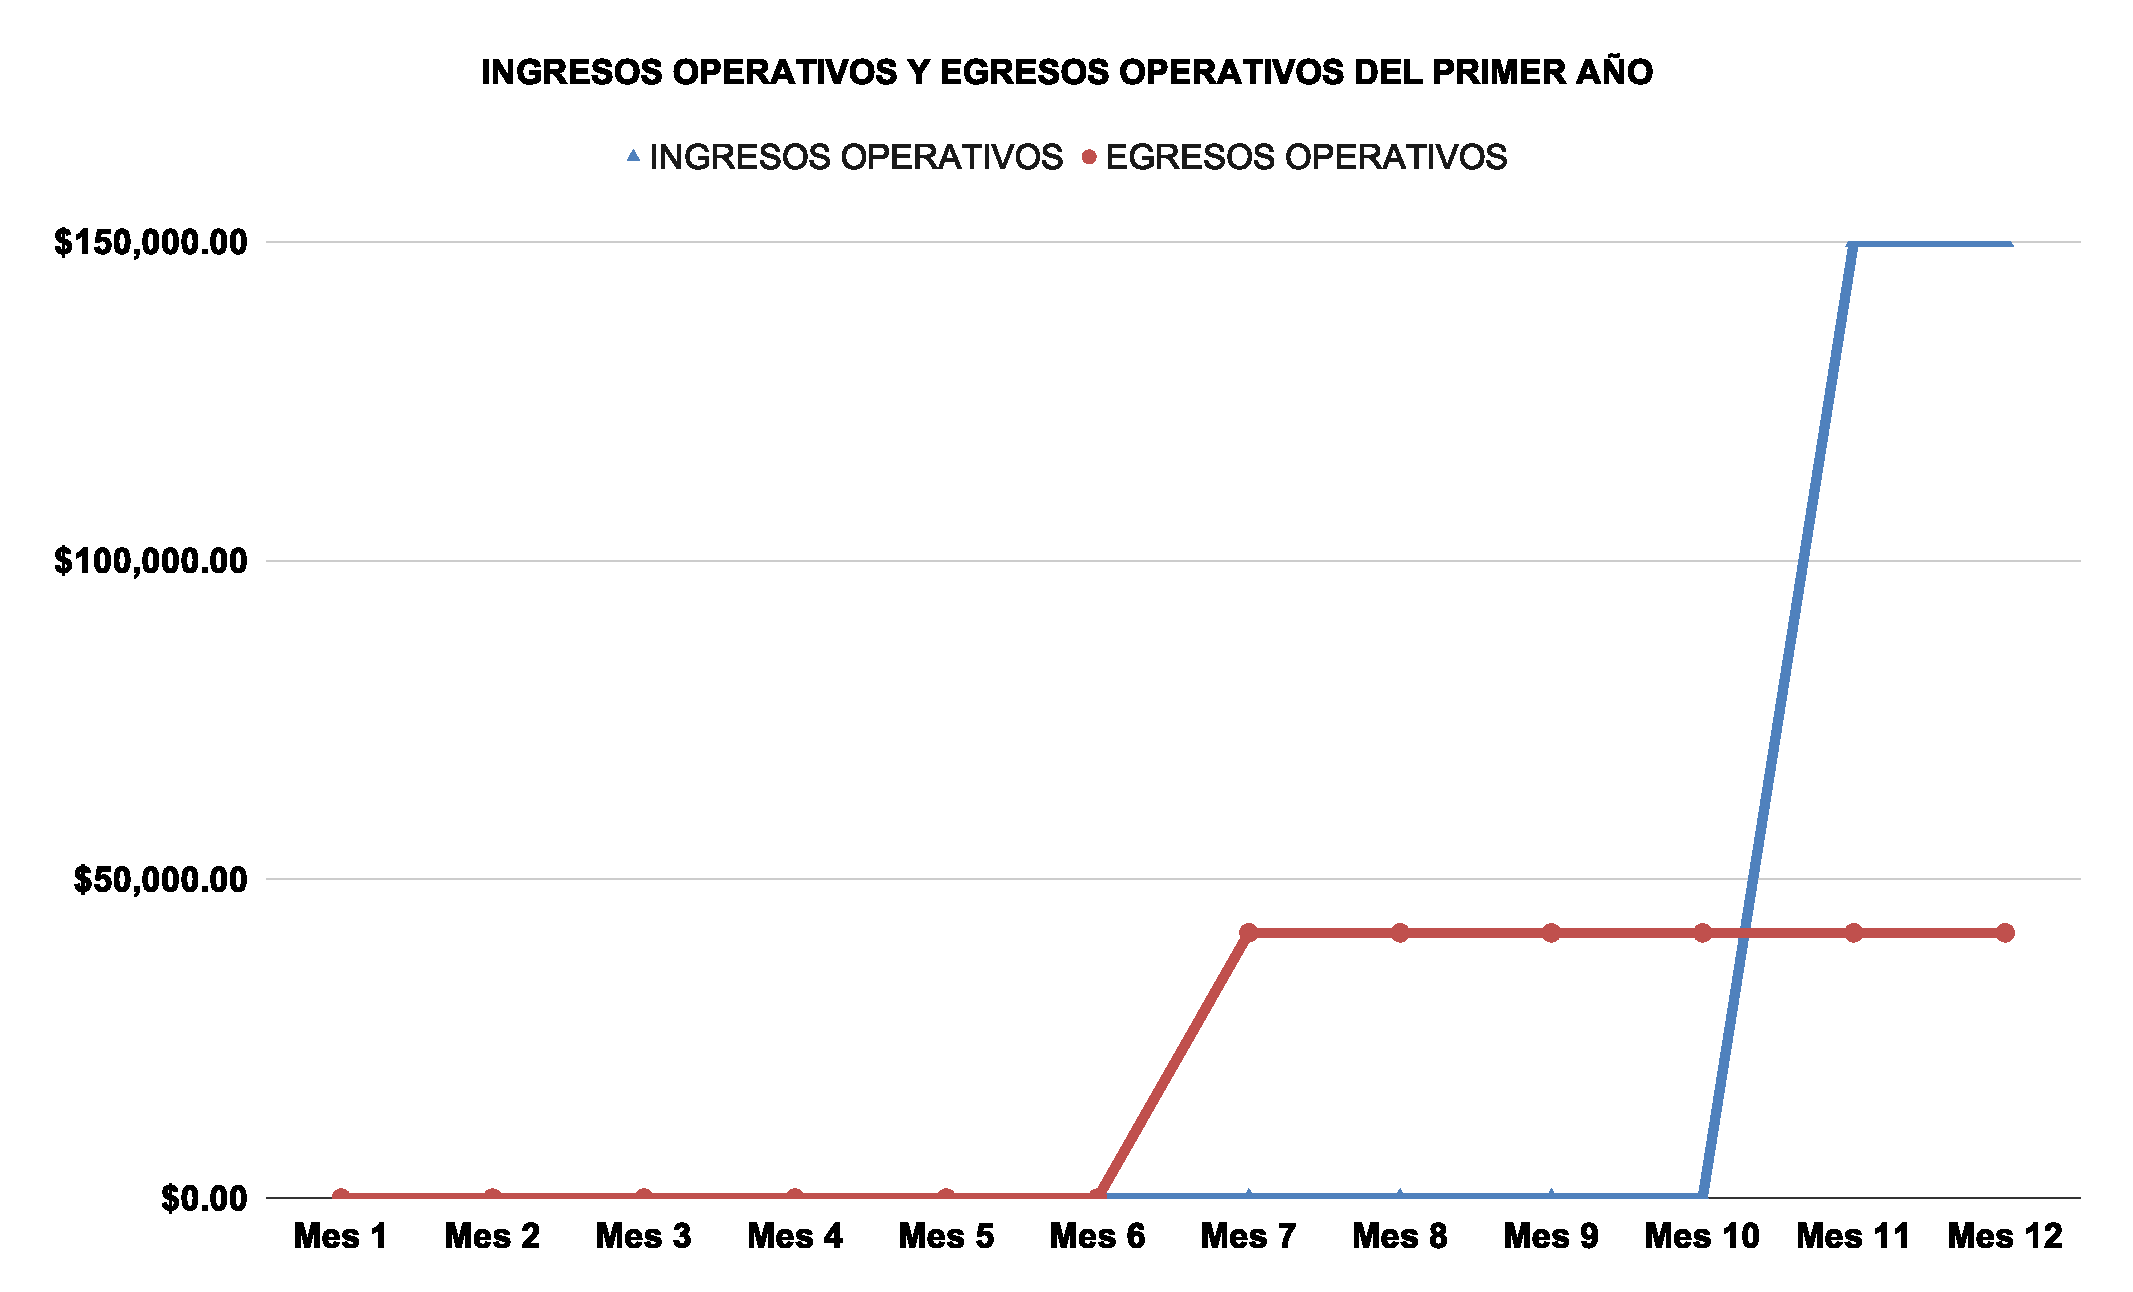
\includegraphics[height=0.28\textheight]{img/flujo_meses_grafico.pdf}}
                \caption{Gráfico de flujo de caja correspondiente a los primeros doce meses.}
            \end{figure}

            \begin{figure}[H]
                \centering
                \makebox[\linewidth][c]{\hspace*{1 cm}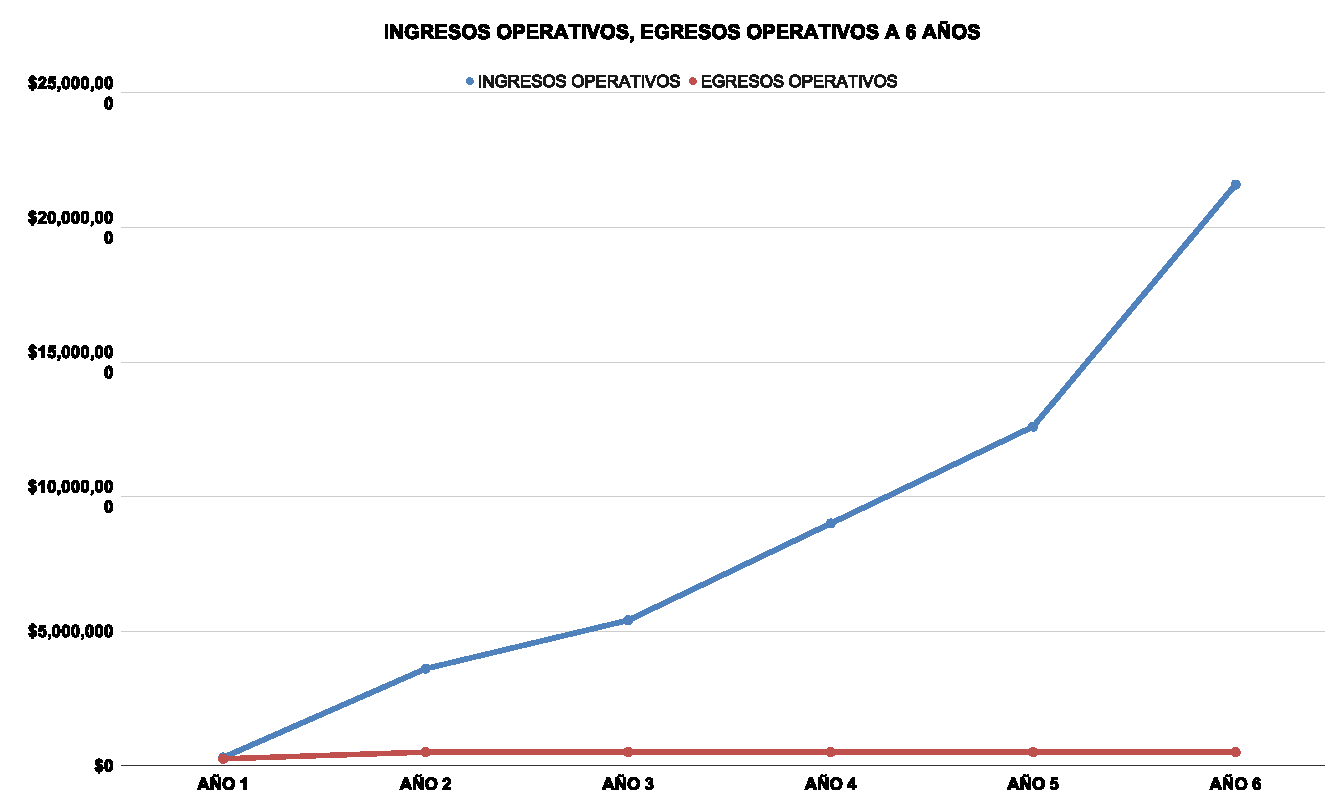
\includegraphics[height=0.28\textheight]{img/flujo_años_grafico.pdf}}
                \caption{Gráfico de flujo de caja correspondiente a los primeros seis años.}
            \end{figure}

            \subsection{Flujo de caja}
                Ver Figuras~\ref{fig:anexo_caja_desarrollo} y \ref{fig:anexo_caja_años} del Anexo.
            
    \phantomsection     
    \section{Gestión de riesgos}

        \phantomsection
        \subsection{Criterios de ponderación}
            
            Para realizar el análisis de riesgos del proyecto, se toma como parámetros de evaluación a los siguientes criterios. En primer lugar, se contempla la probabilidad de ocurrencia de los riesgos mostrada en la Tabla~\ref{riesgos_prob}.
    
                \begin{longtblr}[
                    caption = Escala de probabilidad de ocurrencia de riesgos,
                    label = riesgos_prob
                    ]{
                        cells={ valign = m , halign = c }, 
                        colspec = {Q Q Q[l]}, 
                        rowsep = 4 pt,        
                        colsep = 5 pt,           
                        hlines,              
                        vlines,                             
                        row{1}={bg=gray!15, font=\bfseries, halign = c}
                    }
            
                        Cualitativa & Cuantitativa & Descripción \\ 
                        
                        Recurrente  & 5 & Este riesgo ocurrirá en algún momento \\
                        Probable    & 4 & Existe una gran probabilidad de que este riesgo ocurra \\
                        Posible     & 3 & Este riesgo podría ocurrir o no, probabilidades de 50/50 \\
                        Inusual     & 2 & Existe una gran probabilidad de que este riesgo no ocurra \\
                        Remota      & 1 & El hecho de que este riesgo ocurra es una posibilidad remota \\
            
                \end{longtblr}
        
            Por otro lado, la gravedad de los mismos dada por la Tabla~\ref{riesgos_grav}.
    
                \begin{longtblr}[
                    caption = Escala de gravedad de ocurrencia de riesgos,
                    label = riesgos_grav
                    ]{
                        cells={ valign = m , halign = c }, 
                        colspec = {Q Q Q[l, 9 cm]}, 
                        rowsep = 4 pt,        
                        colsep = 5 pt,           
                        hlines,              
                        vlines,                             
                        row{1}={bg=gray!15, font=\bfseries, halign = c}
                    }
            
                        Cualitativa & Cuantitativa & Descripción \\ 
                        
                        Catastrófica & 5 & Las consecuencias de este riesgo serán muy perjudiciales y puede resultar difícil recuperarse \\
                        
                        Importante & 4 & Las consecuencias de este riesgo serán significativas y pueden causar daños a largo plazo \\
                        
                        Moderada & 3 & Las consecuencias del riesgo tardarán en mitigarse \\
                        
                        Menor & 2 & Las consecuencias del riesgo se gestionarán con facilidad \\
                        
                        Insignificante & 1 & El riesgo generará pocas consecuencias si ocurriera \\
            
                \end{longtblr}
    
            A partir de estos criterios es posible calcular el impacto de los riesgos realizando la multiplicación de la probabilidad por la gravedad, la escala del impacto se observa en la Tabla~\ref{riesgos_imp}.
            
                \begin{longtblr}[
                    caption = Escala de impacto de riesgos considerando probabilidad y gravedad,
                    label = riesgos_imp
                    ]{
                        cells={ valign = m , halign = c }, 
                        colspec = {Q[2.25 cm] Q[2.25 cm] Q[2.25 cm] Q[2.25 cm] Q[2.25 cm] Q[2.25 cm]}, 
                        rowsep = 2.5 pt,        
                        colsep = 5 pt,           
                        hlines,              
                        vlines,                             
                        row{1}={bg=gray!15, font=\bfseries},
                        column{1}={bg=gray!15, font=\bfseries},
                        cell{2}{2,3,4} = {bg=red!25},
                        cell{2}{5} = {bg=orange!30},
                        cell{2}{6} = {bg=green!25},
                        cell{3}{2,3} = {bg=red!25},
                        cell{3}{4,5} = {bg=orange!30},
                        cell{3}{6} = {bg=green!25},
                        cell{4}{2} = {bg=red!25},
                        cell{4}{3,4} = {bg=orange!30},
                        cell{4}{5,6} = {bg=green!25},
                        cell{5}{2,3} = {bg=orange!30},
                        cell{5}{4,5,6} = {bg=green!25},
                        cell{6}{2,3,4,5,6} = {bg=green!25},
                    }
                
                                & Catastrófica & Importante & Moderada & Menor & Insignificante \\
                    Recurrente  & 25 & 20 & 15 & 10 & 5 \\
                    Probable    & 20 & 16 & 12 & 8  & 4 \\
                    Posible     & 15 & 12 & 9  & 6  & 3 \\
                    Remota      & 10 & 8  & 6  & 4  & 2 \\
                    Inusual     & 5  & 4  & 3  & 2  & 1 \\
                
                \end{longtblr}
        
            La clasificación del impacto se realiza de la siguiente forma:
    
                \begin{itemize}
                    \item \textbf{Bajo (0 al 7):} Es probable que los eventos de bajo riesgo no sucedan y, si suceden, no tendrán consecuencias significativas para el proyecto. Baja prioridad en el plan de gestión de riesgos.
    
                    \item \textbf{Medio (8 al 13):} Los eventos de riesgo medio son una molestia y pueden causar contratiempos en el proyecto. No se deben ignorar estos riesgos, pero tampoco es necesario que sean la principal prioridad.
    
                    \item \textbf{Alto (14 al 25):} Si no se los tiene en cuenta durante la planificación del proyecto, los eventos de alto riesgo pueden hacer que el proyecto fracase. Dado que es probable que estos riesgos ocurran y tengan consecuencias graves, son lo más importante en el plan de gestión de riesgos.
                \end{itemize}

        \phantomsection
        \subsection{Riesgos identificados}
    
            En base a lo mencionado anteriormente, se identificaron los riesgos y su impacto en el proyecto como se puede observar en la Tabla~\ref{riesgos}.

                \vspace{0.2 cm}
                \begin{longtblr}[
                    caption = Riesgos y clasificación de los mismos,
                    label = riesgos
                    ]{
                        cells={ valign = m , halign = c }, 
                        colspec = {Q[1 cm] Q[l] Q[2 cm] Q[2 cm] Q[2 cm] Q[2 cm]}, 
                        rowsep = 2.5 pt,        
                        colsep = 5 pt,           
                        hlines,              
                        vlines,                             
                        row{1}={bg=gray!15, font=\bfseries, halign = c}
                    }
            
                        ID & Riesgo identificado & Ocurrencia & Gravedad & Impacto & Riesgo \\ 
                        
                        R1 & Sesgo y falta de generalización      & 3 & 5 & 15 & Alto  \\
                        R2 & Incompatibilidad de formatos         & 4 & 4 & 20 & Alto  \\
                        R3 & Dificultades con los datos locales   & 4 & 5 & 25 & Alto  \\
                        R4 & Fallas en la integración             & 4 & 2 & 8  & Medio \\
                        R5 & Subestimación de costos              & 4 & 3 & 12 & Medio \\
                        R6 & Demora de la certificación           & 3 & 2 & 6  & Bajo  \\
                        R7 & Resistencia de adopción              & 3 & 2 & 6  & Bajo  \\
                        R8 & Diferencias entre los integrantes    & 2 & 1 & 2  & Bajo  \\
            
                \end{longtblr}
    
        \subsubsection*{Descripción de los riesgos}
    
            \begin{enumerate}[label=\textbf{R\arabic* - }] 
            
                \item \textbf{Sesgo y falta de generalización (Alto)}
                
                    El modelo de inteligencia artificial podría no mantener su eficacia al analizar topografías corneales de pacientes locales, debido a que su entrenamiento inicial se basó predominantemente en \textit{datasets} internacionales, generando falsos negativos o diagnósticos imprecisos.
    
                \item \textbf{Incompatibilidad de formatos (Alto)}
                
                    Riesgo de que los equipos topográficos o tomográficos de las clínicas exporten los estudios en formatos propietarios cerrados, anómalos o con resoluciones variables que el \textit{pipeline} de preprocesamiento del software no pueda interpretar adecuadamente.
    
                \item \textbf{Dificultades con los datos locales (Alto)}
                
                    Dificultad o incapacidad para recolectar las muestras topográficas de centros de salud de Misiones en los plazos establecidos, ya sea por falta de tiempo de los médicos colaboradores o por trabas en el proceso de anonimización, bloqueando la fase de validación clínica local.
    
                \item \textbf{Fallas en la integración (Medio)}
                
                   Aparición de errores técnicos, cuellos de botella o incompatibilidades de software al momento de acoplar el modelo de inferencia (\textit{backend/Python}) con la interfaz de usuario (\textit{frontend/React}) y montarlos de forma conjunta en el servidor VPS.
    
                \item \textbf{Subestimación de costos (Medio)}
                
                   Probabilidad de que el presupuesto planificado se vea superado por variaciones económicas reales, como incrementos imprevistos en las suscripciones a servicios Cloud (Google Colab, VPS), honorarios médicos o     aranceles regulatorios.
    
                \item \textbf{Demora de la certificación (Bajo)}
                
                  Posibilidad de sufrir retrasos burocráticos o administrativos durante el proceso de inscripción y auditoría, lo que postergaría el uso clínico formal del producto sin detener su desarrollo técnico.
    
                \item \textbf{Resistencia de adopción (Bajo) }
                
                  Desconfianza o falta de predisposición por parte de algunos oftalmólogos y técnicos locales para incorporar un sistema de IA como segunda opinión, prefiriendo sus métodos tradicionales y limitando el alcance de las pruebas operativas.
    
                \item \textbf{Diferencias entre los integrantes (Bajo)} 
                
                  Posibles desacuerdos técnicos, de criterio o de disponibilidad de horarios entre los miembros del equipo desarrollador, lo que podría generar pequeñas fricciones o ralentizar momentáneamente el avance de ciertas tareas.
                
            \end{enumerate}

        \phantomsection
        \subsection{Planes de acción}
    
            \begin{enumerate}[label=\textbf{R\arabic* - }] 
            
                \item \textbf{Sesgo y falta de generalización (Alto)}
                
                    \textbf{Mitigación:} Se implementarán técnicas de \textit{Data Augmentation} (aumento de datos) para enriquecer artificialmente las muestras locales disponibles, mejorando la robustez del modelo de \textit{Deep Learning}. Además se implementará seguimiento al entrenamiento para prevenir \textit{overfitting} y \textit{underfitting} de los datos internacionales disponibles así como reentrenamiento continuo y monitoreo de deriva.
    
                    \textbf{Contingencia:} En caso de detectar un alto índice de falsos negativos durante las pruebas, se programarán sesiones intensivas con el oftalmólogo consultor para analizar exclusivamente los mapas de calor (XAI) de los casos erróneos. Esto permitirá identificar qué patrones morfológicos sutiles está ignorando la IA para proceder a un reentrenamiento focalizado y ajuste de la clasificación.
    
                \item \textbf{Incompatibilidad de formatos (Alto)}
    
                    \textbf{Mitigación:} Desde las fases iniciales, se solicitarán muestras de prueba de los distintos equipos disponibles en el mercado local (Pentacam). Con base en estas muestras, se construirá un \textit{pipeline} de preprocesamiento robusto en Python utilizando herramientas de visión artificial.
    
                    \textbf{Contingencia:} Si se detectan resoluciones anómalas o escalas de color propietarias que rompan la segmentación, el módulo de preprocesamiento se actualizará para forzar una estandarización (recorte, redimensionamiento y normalización de canales) antes de que la imagen ingrese al modelo predictivo, asegurando así la interoperabilidad del sistema.
                
                \item \textbf{Dificultades con los datos locales (Alto)}
    
                    \textbf{Mitigación:} Se desarrollará y entregará a los oftalmólogos colaboradores un \textit{script} automatizado y sencillo que elimine de manera instantánea los metadatos (información del paciente) de las imágenes exportadas. Esto reducirá drásticamente la carga de trabajo administrativo para ellos al momento de anonimizar las muestras.
    
                    \textbf{Contingencia:} Si un único centro médico no logra alcanzar la cuota de imágenes necesarias en el tiempo estimado, se ampliará inmediatamente la solicitud de colaboración a otras clínicas oftalmológicas o centros de alta complejidad ubicados en los principales núcleos urbanos de la provincia de Misiones (como Posadas, Oberá y Eldorado).
                
                \item \textbf{Fallas en la integración (Medio)}
    
                    \textbf{Mitigación:} El desarrollo se realizará de manera estrictamente modular. Se construirán y probarán de forma aislada los \textit{endpoints} de la API en el \textit{backend} antes de conectarlos a la interfaz gráfica desarrollada en React.
    
                    \textbf{Contingencia:} Se utilizarán tecnologías de contenerización (como Docker) para encapsular la aplicación. De este modo, si surgen incompatibilidades al migrar el sistema desde las computadoras de desarrollo local hacia el servidor VPS, el contenedor garantizará que el entorno de ejecución sea exactamente el mismo, aislando el problema rápidamente.
                       
                \item \textbf{Subestimación de costos (Medio)}
    
                    \textbf{Mitigación:} Se llevará un control estricto de los gastos operativos y se optimizará el uso de la infraestructura en la nube (activando los recursos de pago como Google Colab Pro solo en periodos críticos). Para contener los gastos en honorarios médicos durante la auditoría de datos, se buscará establecer convenios de colaboración académica con los especialistas locales, ofreciendo coautoría en publicaciones científicas a cambio de su asesoramiento experto.
    
                    \textbf{Contingencia:} En caso de que los aranceles regulatorios (como la habilitación de empresa y registro del producto médico ante la ANMAT) superen la capacidad financiera del proyecto, se buscará una asociación estratégica con una institución médica o empresa tecnológica que ya posea la habilitación legal correspondiente. Alternativamente, la primera versión se podría distribuir como software de uso para investigación (\textit{Research Use Only}) sin validez diagnóstica comercial, lo que evitará los altos costos de registro inicial hasta que se consiga financiamiento externo o rondas de inversión.
                    
            \end{enumerate}

        \phantomsection
        \subsection{Impacto temporal}

            La materialización de los riesgos identificados afecta de forma distinta al cronograma del proyecto, existiendo casos donde el impacto es directo, otros donde es indirecto o acotado, y otros donde no compromete la planificación técnica.
            
            En el caso de \textbf{R1 (Sesgo y falta de generalización)}, si se detecta durante la etapa de validación clínica, la contingencia de reentrenamiento focalizado implicaría un retroceso hacia la etapa de desarrollo, extendiendo su duración original. De forma similar, \textbf{R2 (Incompatibilidad de formatos)} puede afectar el cronograma en dos momentos distintos: durante el desarrollo, si obliga a reconstruir el módulo de preprocesamiento antes de continuar con el entrenamiento, o durante la validación clínica local, si algún centro de salud utiliza un equipo con un formato no contemplado originalmente, retrasando el inicio de esa etapa. 
            
            \textbf{R3 (Dificultades con los datos locales)} constituye el caso más directo, ya que su propia definición está condicionada por los plazos de recolección y su materialización bloquea explícitamente el comienzo de la etapa de validación clínica local hasta resolverse. En contraste, \textbf{R4 (Fallas en la integración)} presenta un impacto temporal acotado, dado que el desarrollo modular y la contenerización mediante Docker permiten aislar y resolver los errores rápidamente sin detener el avance general del proyecto. 
            
            \textbf{R5 (Subestimación de costos)} impacta principalmente en lo financiero y no en el cronograma técnico de desarrollo. Sin embargo, puede generar una afectación indirecta si se activa su contingencia, ya que gestionar una asociación estratégica o una ronda de financiamiento externo consume tiempo adicional que podría postergar puntualmente la etapa de certificación regulatoria y lanzamiento.
            
            \textbf{R6 (Demora de la certificación)} no afecta el cronograma de desarrollo técnico, ya que su propia descripción aclara que los retrasos burocráticos posponen únicamente el uso clínico formal y comercial del producto, permitiendo que el desarrollo continúe en paralelo. 
            
            \textbf{R7 (Resistencia de adopción)} recae más sobre el alcance que sobre el tiempo, reduciendo la cantidad de casos disponibles durante la validación en lugar de extender directamente su duración, salvo que sea necesario reclutar centros o profesionales adicionales, lo que generaría una demora acotada. 
            
            Finalmente, \textbf{R8 (Diferencias entre los integrantes)} sí presenta una afectación sobre el cronograma según su propia descripción, aunque de carácter menor, puntual y limitado a tareas específicas del equipo, sin comprometer las etapas generales del proyecto.

            En conclusión, los riesgos con afectación directa y relevante sobre el cronograma son \textbf{R1, R2 y R3}, los riesgos con afectación indirecta o acotada son \textbf{R4, R5, R7 y R8}, mientras que \textbf{R6} es el único riesgo que no compromete en ningún grado el desarrollo técnico ni su cronograma.